
%\begin{center}

      \pagestyle{empty}


~

\vspace{-5mm}

\hspace{-9mm}
\framebox[1.05\width]{

  \begin{minipage}[t][25cm]{16cm}  %% 24 cm
  \rule{0cm}{5mm}

  \vspace{-.3cm}
  \large  \hfill BNL (2011) \\[-.5cm]

  \vfill
  \vspace{-2cm}
  \title{ 
      \textbf{
              \huge ZGOUBI USERS' GUIDE     \\
                  ~                          \\
              \large ZGOUBI ON WEB~: \\ http://sourceforge.net/projects/zgoubi/
             }    
        }

    \author{ 
             \textbf{Fran\c{c}ois M\'eot }                      \\[0ex]
             { \em Brookhaven National Laboratory   }             \\[-.9ex]
             {\em Collider-Accelerator Department   }            \\[-.9ex]
             { \em Upton, NY, 11973 }           
           }

    \maketitle

  \vfill  %space{2cm}

    \date

    \vfill


      { \hspace{36mm} LHC IP \hspace{45mm} Snake Resonance Crossing, RHIC \hfill } \\[1ex]
    %
    \centerline{
      \mbox{
         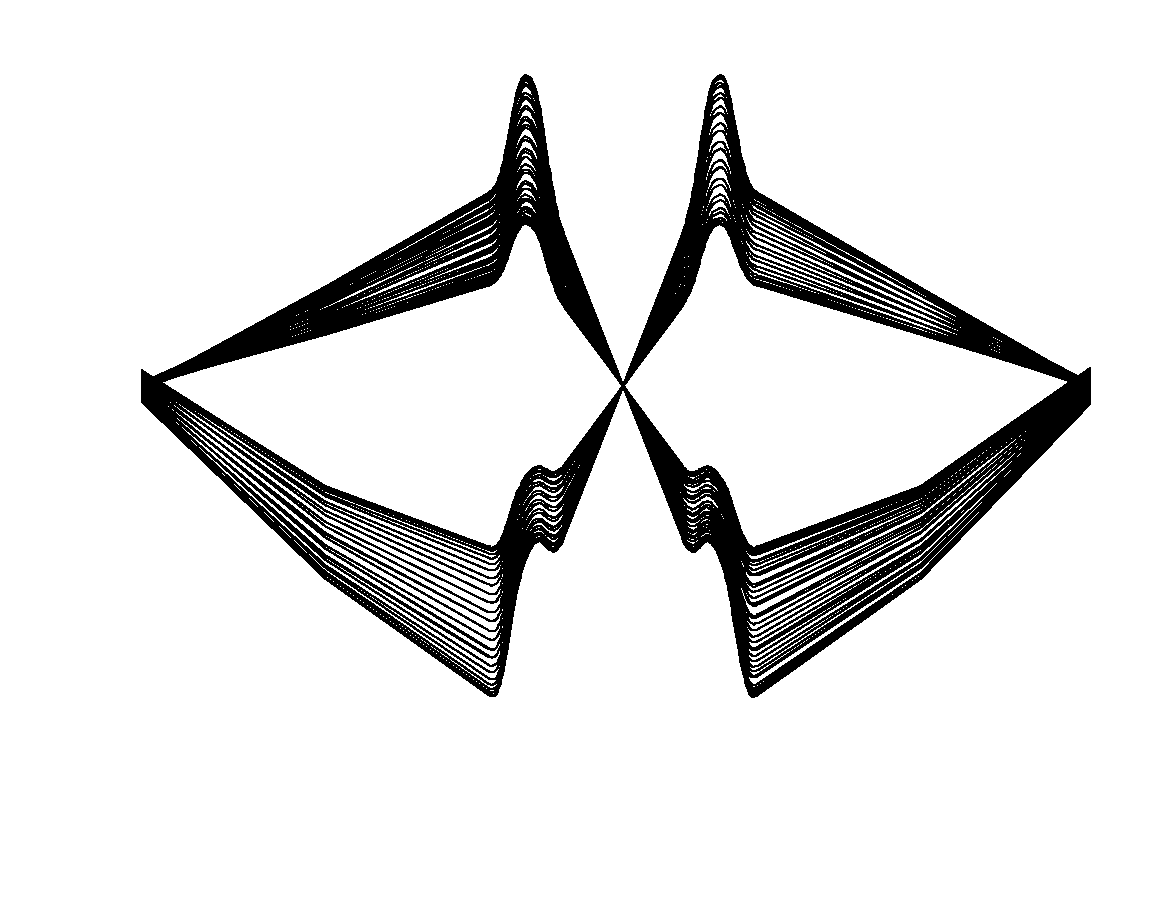
\includegraphics[width=10cm]{FigCover1.ps}
          \hspace{2ex}
         \includegraphics[width=9cm,height=5cm]{FigCover2New.ps} 
       }
     }


      {  \hspace{25mm} Spin Flip, AGS Cycle \hspace{41mm} DA, Muon Decay Ring \hfill } \\[1.2ex]
     %
    \centerline{
      \mbox{
         \hspace{0mm}
         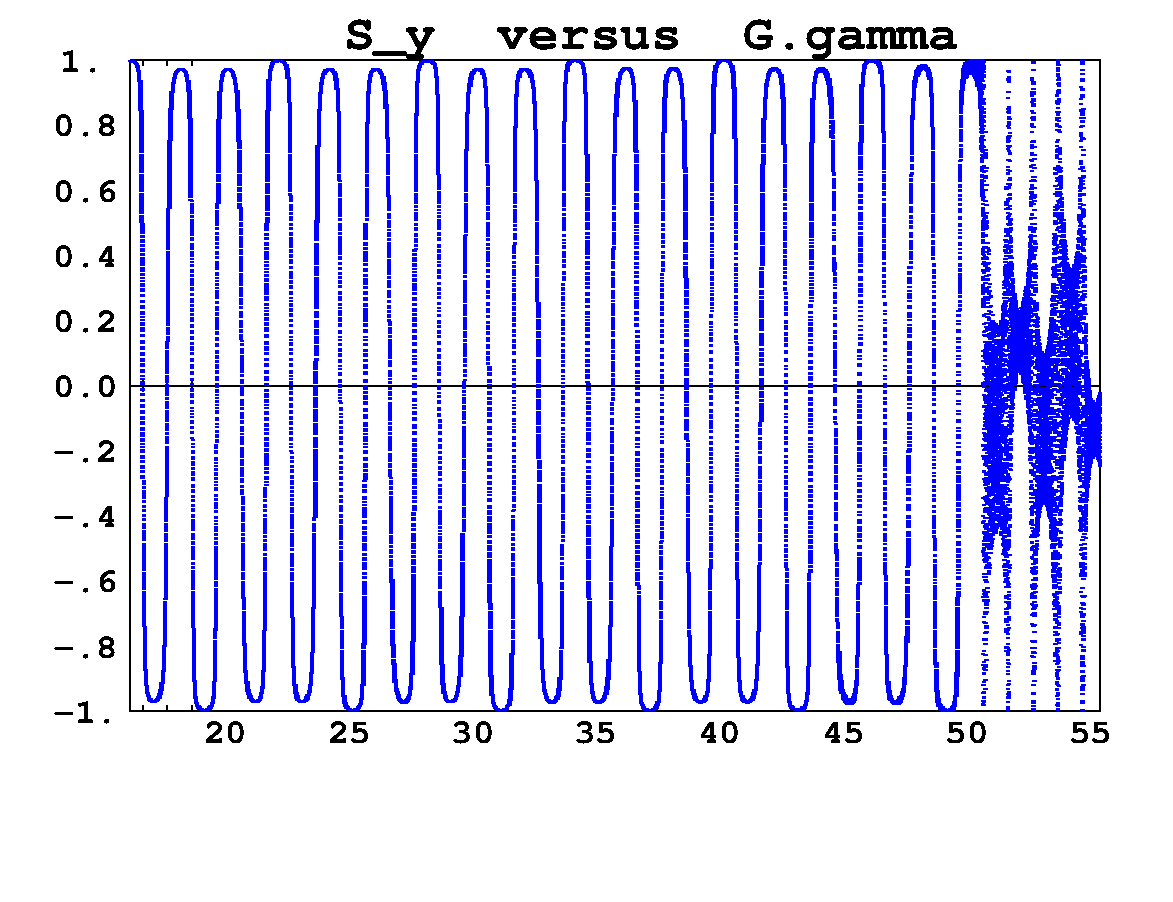
\includegraphics[width=7.2cm]{FigCover3New.ps}
         \hspace{12mm}
         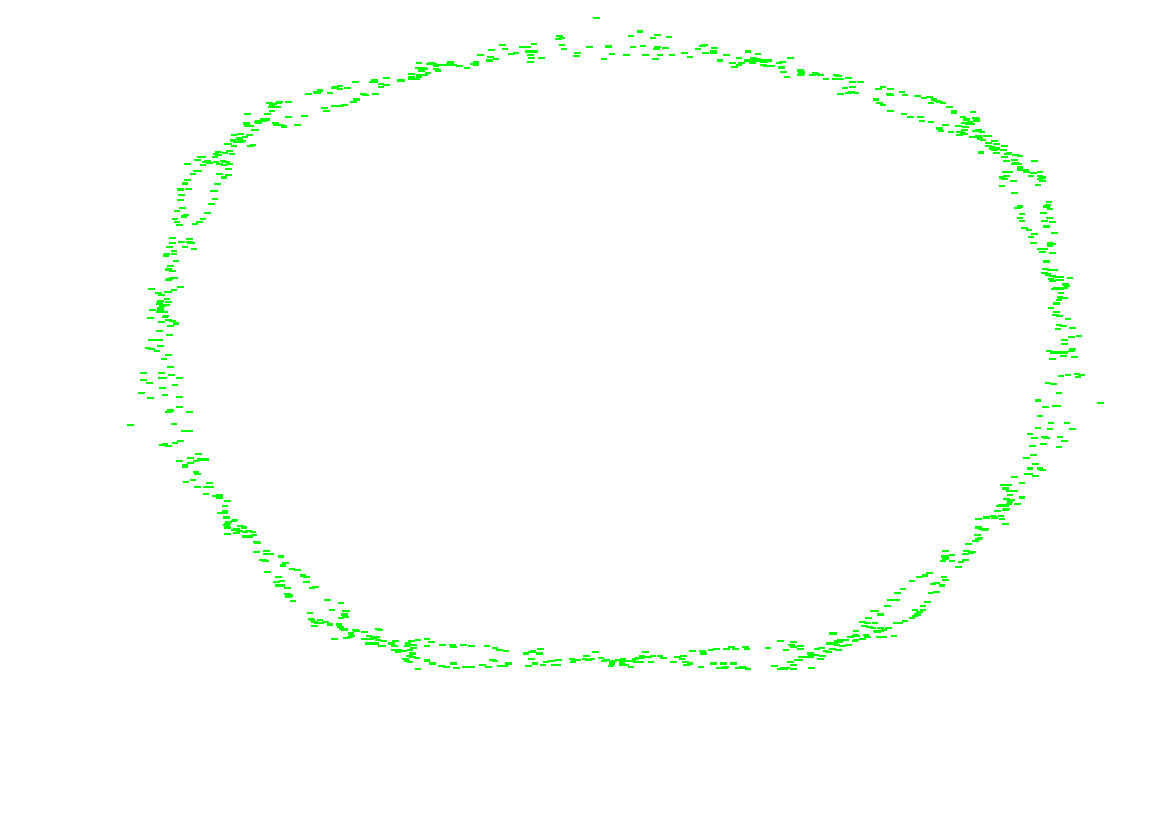
\includegraphics[width=7cm]{FigCover4.ps}
       }
     }

  \end{minipage}
}
%\end{center}


\newpage


~~~~~~~~~~~
  \footnotetext{\Large  {\bf Cover figures} :  \\
  {\it upper left} : collision optics at ATLAS and CMS, \\
  {\it upper right} : polarization upon crossing of 393+$Q_y$ resonance in RHIC,  \\
  {\it lower left} : spin-flipping with partial snakes along AGS cycle,   \\
  {\it lower right} : dynamic aperture in the Neutrino Factory muon decay ring.
   }

